\documentclass[12pt,openany]{book}

% ============================================================
% Livro de Notas de Aula (Professor)
% Pasta: aed/aula/
% Objetivo: compilar direto no Overleaf como um livro separado.
% ============================================================

\usepackage[a4paper,margin=2.5cm]{geometry}
\usepackage[T1]{fontenc}
\usepackage[utf8]{inputenc}
\usepackage[brazil]{babel}
\usepackage{lmodern}
\usepackage{microtype}
\usepackage{amsmath, amssymb, amsthm}
\usepackage{booktabs}
\usepackage{graphicx}
\usepackage{xcolor}
\usepackage{hyperref}
\usepackage{enumitem}
\usepackage{array}
\usepackage{float}
\usepackage{caption}
\usepackage{listings}
\usepackage{siunitx}
\usepackage[most]{tcolorbox}

\hypersetup{colorlinks=true,linkcolor=blue,urlcolor=blue,citecolor=teal}

% ---------- Colors (pastel palette) ----------
\definecolor{pastelblue}{HTML}{E6F0FF}
\definecolor{pastelgray}{HTML}{F2F2F2}
\definecolor{pastelorange}{HTML}{FFEBD6}
\definecolor{pastelteal}{HTML}{DFF7F2}

% "Verde quadro" (fundo claro + borda/realce)
\definecolor{boardgreen}{HTML}{0B3D2E}
\definecolor{boardgreenlight}{HTML}{E9F6EF}

% ---------- tcolorbox styles ----------
\tcbset{sharp corners, boxrule=0pt, coltitle=black, fonttitle=\bfseries, left=8pt, right=8pt, top=6pt, bottom=6pt}

\newtcolorbox{FormulaBox}[1][]{colback=pastelblue, coltitle=white, title=Fórmula, #1}
\newtcolorbox{ProofBox}[1][]{colback=pastelgray, coltitle=white, title=Demonstração (Resumo), #1}
\newtcolorbox{SolvedBox}[1][]{colback=pastelorange, coltitle=white, title=Checklist / Entrega, #1}
\newtcolorbox{NoteBox}[1][]{colback=pastelteal, coltitle=white, title=Nota, #1}

% Caixa "No Quadro" (verde)
\newtcolorbox{BoardBox}[1][]{
  colback=boardgreenlight,
  colframe=boardgreen,
  boxrule=0.6pt,
  title=No Quadro,
  coltitle=white,
  fonttitle=\bfseries,
  #1
}

% ---------- Listings (Python & SQL) ----------
\lstdefinestyle{codeblock}{
  basicstyle=\ttfamily\small,
  numbers=left,
  numberstyle=\tiny,
  stepnumber=1,
  numbersep=6pt,
  showstringspaces=false,
  breaklines=true,
  frame=single,
  framerule=0.2pt,
  framesep=6pt,
  rulecolor=\color{pastelgray},
  xleftmargin=1em,
  xrightmargin=1em
}
\lstdefinelanguage{SQL}{morekeywords={SELECT,FROM,WHERE,AND,OR,JOIN,LEFT,RIGHT,INNER,OUTER,ON,AS,GROUP,BY,ORDER,INSERT,INTO,VALUES,UPDATE,DELETE,CREATE,TABLE,VIEW,DROP,ALTER,PRIMARY,KEY,NOT,NULL,DEFAULT,DISTINCT}, sensitive=false}
\lstset{style=codeblock}

% ---------- Bibliografia ----------
% Observação: manter estilo amplamente suportado no Overleaf.
\usepackage[backend=biber,style=authoryear]{biblatex}
\addbibresource{referencias.bib}

\title{\Huge \textbf{Notas de Aula (Professor)}\\ \Large AED, Python, Tableau e Storytelling (2026.1)}
\author{Cayo Oliveira}
\date{2026}

\begin{document}
\maketitle
\tableofcontents

% ------------------------------------------------------------
% Parte 0: Plano (mesmo conteúdo do plano.tex)
% ------------------------------------------------------------

\documentclass[12pt]{article}

\usepackage[a4paper,margin=2.5cm]{geometry}
\usepackage[T1]{fontenc}
\usepackage[utf8]{inputenc}
\usepackage[brazil]{babel}
\usepackage{lmodern}
\usepackage{microtype}
\usepackage{amsmath, amssymb}
\usepackage{booktabs}
\usepackage{array}
\usepackage{xcolor}
\usepackage{hyperref}
\usepackage{enumitem}
\usepackage[most]{tcolorbox}

\hypersetup{colorlinks=true,linkcolor=blue,urlcolor=blue,citecolor=teal}

% ---------- Colors (pastel palette) ----------
\definecolor{pastelblue}{HTML}{E6F0FF}
\definecolor{pastelgray}{HTML}{F2F2F2}
\definecolor{pastelorange}{HTML}{FFEBD6}
\definecolor{pastelteal}{HTML}{DFF7F2}

% ---------- tcolorbox styles (compatível com o livro) ----------
\tcbset{sharp corners, boxrule=0pt, coltitle=black, fonttitle=\bfseries, left=8pt, right=8pt, top=6pt, bottom=6pt}

\newtcolorbox{NoteBox}[1][]{colback=pastelteal, coltitle=white, title=Nota, #1}
\newtcolorbox{SolvedBox}[1][]{colback=pastelorange, coltitle=white, title=Entrega (Checklist), #1}

\title{\Huge \textbf{Plano de Ensino}\\ \Large Análise Exploratória de Dados e Storytelling (2026.1)}
\author{Sistemas de Informação -- UNIFACOL}
\date{Fevereiro -- Maio/Junho de 2026}

\begin{document}
\maketitle

\section{Visão Geral}
Esta disciplina tem dois objetivos complementares:
\begin{itemize}[leftmargin=*]
	\item \textbf{Unidade I (semanas 01--07):} construir a base de \textbf{AED} com \textbf{estatística prática} e \textbf{Python (Pandas)} para limpar, resumir e interpretar dados;
	\item \textbf{Unidade II (semanas 08--12):} transformar insights em \textbf{comunicação persuasiva} com \textbf{Tableau} e \textbf{storytelling}.
\end{itemize}

\begin{NoteBox}
\textbf{Regra do ritmo (aula noturna 19h--22h):} em semanas com trabalho, as \textbf{apresentações ocupam no máximo 1 hora}. O restante da aula continua com teoria + prática guiada.
\end{NoteBox}

\section{Calendário Letivo (12 semanas de aula)}
O calendário abaixo está alinhado ao arquivo \texttt{aed/calendario.md}. Semanas marcadas como \textit{não conta} (feriados/provas) não entram na contagem das 12 semanas.

\begin{center}
\renewcommand{\arraystretch}{1.15}
\begin{tabular}{@{}c p{3.2cm} p{4.2cm} p{5.7cm}@{}}
\toprule
\textbf{Semana} & \textbf{Período (Seg--Qua)} & \textbf{Tipo da semana} & \textbf{Observação} \\
\midrule
01 & 02/02 a 04/02 & Teoria + lab & Início das aulas \\
02 & 09/02 a 11/02 & Teoria + \textbf{Trabalho 1} & Entrega quinzenal \\
\midrule
\multicolumn{4}{@{}l}{\textit{14 a 18/02 --- Carnaval [F] (não conta semana)}}\\
\midrule
03 & 23/02 a 25/02 & Teoria + lab & Semana normal \\
04 & 02/03 a 04/03 & Teoria + \textbf{Trabalho 2} & Entrega quinzenal \\
05 & 09/03 a 11/03 & Teoria + lab & Semana normal \\
06 & 16/03 a 18/03 & Teoria + \textbf{Trabalho 3} & Entrega quinzenal \\
07 & 23/03 a 25/03 & Teoria + lab & Semana normal \\
\midrule
\multicolumn{4}{@{}l}{\textit{02 a 04/04 --- Semana Santa [F] (não conta semana)}}\\
\multicolumn{4}{@{}l}{\textit{06 a 14/04 --- Prova I Unidade (não conta semana)}}\\
\midrule
08 & 20/04 & Teoria + \textbf{Trabalho 4} & Aula apenas na segunda (21/04 é feriado) \\
09 & 27/04 a 29/04 & Teoria + lab & Semana normal \\
10 & 04/05 a 06/05 & Teoria + \textbf{Trabalho 5} & 06/05 é feriado (Vitória) \\
11 & 11/05 a 13/05 & Teoria + lab & Semana normal \\
12 & 18/05 a 20/05 & Teoria + \textbf{Trabalho 6} & Entrega quinzenal (encerramento do conteúdo) \\
\midrule
\multicolumn{4}{@{}l}{\textit{25/05 a 01/06 --- Prova II Unidade (não conta semana)}}\\
\bottomrule
\end{tabular}
\end{center}

\section{Avaliação (visão operacional)}
\begin{itemize}[leftmargin=*]
	\item \textbf{Trabalhos quinzenais (T1--T6):} entregas práticas curtas, com apresentação e checklist.
	\item \textbf{Prova I Unidade:} janela 06/04 a 14/04 (conforme calendário institucional).
	\item \textbf{Prova II Unidade:} janela 25/05 a 01/06.
\end{itemize}

\begin{NoteBox}
\textbf{Formato padrão de entrega (em todos os trabalhos):}
\begin{itemize}[leftmargin=*]
	\item \textbf{Python}: 1 notebook com ETL + checagens (tipos, ausências, duplicadas, filtros).
	\item \textbf{Dados}: 1 CSV ``limpo'' pronto para visualização.
	\item \textbf{Tableau}: 1 workbook (ou export) com visuais/dash.
	\item \textbf{Comunicação}: 1 slide (ou texto curto) com \textbf{Big Idea} + 3 bullets de evidências.
\end{itemize}
\end{NoteBox}

\section{Plano Semana a Semana (conteúdo + aprendizagem + entregas)}

\subsection*{Semana 01 (02/02--04/02) --- Do Caos à Clareza: AED e a \textit{Big Idea}}
\textbf{O que vai ter na semana:}
\begin{itemize}[leftmargin=*]
	\item Abertura com \textbf{gancho} e \textbf{Big Idea} do semestre: ``dados brutos são ruído; valor é extrair uma história que force uma decisão''.
	\item Diferença entre \textbf{análise exploratória} (cozinha) e \textbf{análise explanativa} (jantar).
	\item Primeiro \textbf{ETL com Python/Pandas}: leitura, inspeção, tipos, ausências, conversão de datas, remoção de colunas e exportação de CSV limpo.
	\item Primeiro contato com \textbf{Tableau}: conectar CSV e gerar visuais rápidos.
	\item Design básico: \textbf{Teste do Relance (3 segundos)} e remoção de ``lixo visual''.
\end{itemize}

\textbf{O aluno aprende a:}
\begin{itemize}[leftmargin=*]
	\item Diferenciar \textbf{descobrir} insight (AED) de \textbf{comunicar} insight (storytelling).
	\item Rodar um ETL simples e produzir um dataset ``pronto para viz''.
	\item Construir o primeiro visual no Tableau e avaliar clareza pelo Teste do Relance.
\end{itemize}

\begin{SolvedBox}
\textbf{Preparação para o Trabalho 1 (entrega na Semana 02):}
\begin{itemize}[leftmargin=*]
	\item Escolher um dataset simples (Kaggle ou base sugerida pelo professor).
	\item Definir 1 pergunta de negócio e 1 Big Idea.
\end{itemize}
\end{SolvedBox}

\subsection*{Semana 02 (09/02--11/02) --- Trabalho 1 (apresentações) + Fundamentos de dados retangulares}
\textbf{Formato da aula:}
\begin{itemize}[leftmargin=*]
	\item \textbf{Até 1 hora}: apresentações relâmpago do T1 (2--3 min por aluno/grupo).
	\item \textbf{Restante}: teoria + prática guiada.
\end{itemize}

\textbf{Teoria/Prática da semana:}
\begin{itemize}[leftmargin=*]
	\item \textbf{Dados retangulares}: linhas x colunas, variável x registro.
	\item \textbf{Dicionário de dados} e perguntas: ``o que cada coluna significa?''.
	\item Qualidade básica: ausências, duplicadas, categorias sujas, datas e textos.
\end{itemize}

\textbf{O aluno aprende a:}
\begin{itemize}[leftmargin=*]
	\item Formular uma pergunta e traduzir em colunas/transformações.
	\item Entregar uma história curta com evidência (Big Idea + visuais).
\end{itemize}

\begin{SolvedBox}
\textbf{Trabalho 1 (entrega na Semana 02):} ETL básico + \textbf{3 visuais} no Tableau + Big Idea (1 slide).
\end{SolvedBox}

\subsection*{Semana 03 (23/02--25/02) --- Estatística descritiva I: medidas de posição}
\textbf{O que vai ter na semana:}
\begin{itemize}[leftmargin=*]
	\item \textbf{Média, mediana, moda} e quando usar cada uma.
	\item \textbf{Resumo com Pandas}: \texttt{describe}, \texttt{value\_counts}, \texttt{groupby}.
	\item Leitura crítica: por que ``média'' pode mentir (assimetria/outliers).
\end{itemize}

\textbf{O aluno aprende a:}
\begin{itemize}[leftmargin=*]
	\item Resumir uma coluna numérica e uma coluna categórica.
	\item Explicar em linguagem de negócio o que um resumo indica.
\end{itemize}

\subsection*{Semana 04 (02/03--04/03) --- Trabalho 2 (apresentações) + Estatística descritiva II: variabilidade}
\textbf{Formato da aula:}
\begin{itemize}[leftmargin=*]
	\item \textbf{Até 1 hora}: apresentações do T2.
	\item \textbf{Restante}: teoria + prática (boxplot, IQR, dispersão).
\end{itemize}

\textbf{Teoria/Prática da semana:}
\begin{itemize}[leftmargin=*]
	\item \textbf{Variância, desvio-padrão, amplitude, IQR} e leitura prática.
	\item \textbf{Outliers}: por que aparecem e como investigar antes de remover.
\end{itemize}

\textbf{O aluno aprende a:}
\begin{itemize}[leftmargin=*]
	\item Comparar dois grupos (ex.: por categoria) usando medidas de posição e dispersão.
	\item Justificar escolhas (mediana vs média; IQR vs DP) com base no dado.
\end{itemize}

\begin{SolvedBox}
\textbf{Trabalho 2 (entrega na Semana 04):} mini-relatório AED (posição + dispersão) + 2 visuais (boxplot + histograma) + Big Idea.
\end{SolvedBox}

\subsection*{Semana 05 (09/03--11/03) --- Distribuições e dados ausentes: o ``formato'' dos dados}
\textbf{O que vai ter na semana:}
\begin{itemize}[leftmargin=*]
	\item \textbf{Histogramas} e leitura de forma (simetria/assimetria; caudas).
	\item \textbf{Valores ausentes}: tipos de missing e estratégias (imputar, remover, sinalizar).
	\item \textbf{Regras práticas} para preparar dados para o Tableau (tipos, datas, categorias).
\end{itemize}

\textbf{O aluno aprende a:}
\begin{itemize}[leftmargin=*]
	\item Identificar distribuições problemáticas e propor transformações simples.
	\item Tratar missing sem ``matar'' o significado do dado.
\end{itemize}

\subsection*{Semana 06 (16/03--18/03) --- Trabalho 3 (apresentações) + Correlação introdutória}
\textbf{Formato da aula:}
\begin{itemize}[leftmargin=*]
	\item \textbf{Até 1 hora}: apresentações do T3.
	\item \textbf{Restante}: teoria + prática (correlação e gráficos bivariados).
\end{itemize}

\textbf{Teoria/Prática da semana:}
\begin{itemize}[leftmargin=*]
	\item \textbf{Dispersão (scatter)} e o que \textbf{correlação} mede (e o que não mede).
	\item \textbf{Segmentação} por categoria (cor por classe, facetas simples).
\end{itemize}

\textbf{O aluno aprende a:}
\begin{itemize}[leftmargin=*]
	\item Investigar relações entre duas variáveis sem cair em conclusões causais.
	\item Contar uma história com evidência bivariada (2 visuais coerentes).
\end{itemize}

\begin{SolvedBox}
\textbf{Trabalho 3 (entrega na Semana 06):} diagnóstico (missing + outliers + distribuição) + 1 relação bivariada (scatter) + Big Idea.
\end{SolvedBox}

\subsection*{Semana 07 (23/03--25/03) --- Variáveis categóricas e revisão para Prova I}
\textbf{O que vai ter na semana:}
\begin{itemize}[leftmargin=*]
	\item \textbf{Categóricas}: proporções, tabelas de frequência e gráficos de barras.
	\item \textbf{Boas práticas} de escolha de gráfico (evitar pizza quando não faz sentido).
	\item Revisão guiada dos conceitos da Unidade I (ETL, resumos, distribuições, correlação).
\end{itemize}

\textbf{O aluno aprende a:}
\begin{itemize}[leftmargin=*]
	\item Comparar categorias com clareza e consistência visual.
	\item Consolidar um ``kit'' de AED para a Prova I.
\end{itemize}

\subsection*{Semana 08 (20/04) --- Trabalho 4 (apresentações) + Storytelling: da análise à decisão}
\textbf{Observação:} aula concentrada (apenas segunda-feira).

\textbf{Formato da aula:}
\begin{itemize}[leftmargin=*]
	\item \textbf{Até 1 hora}: apresentações do T4.
	\item \textbf{Restante}: storytelling aplicado (estrutura e mensagem).
\end{itemize}

\textbf{Teoria/Prática da semana:}
\begin{itemize}[leftmargin=*]
	\item \textbf{AED vs explanativa} (retomada): o que entra e o que não entra numa apresentação.
	\item \textbf{Big Idea} e \textbf{pergunta de decisão}: ``o que eu quero que a audiência faça?''
	\item Primeiro \textbf{storyboard} (3 a 5 telas) para um dashboard.
\end{itemize}

\textbf{O aluno aprende a:}
\begin{itemize}[leftmargin=*]
	\item Transformar achados em uma linha narrativa curta.
	\item Planejar um dashboard antes de construir.
\end{itemize}

\begin{SolvedBox}
\textbf{Trabalho 4 (entrega na Semana 08):} roteiro curto (Big Idea + 3 evidências) + esboço de dashboard (wireframe) + 1 visual no Tableau.
\end{SolvedBox}

\subsection*{Semana 09 (27/04--29/04) --- Design de informação: clareza, hierarquia e consistência}
\textbf{O que vai ter na semana:}
\begin{itemize}[leftmargin=*]
	\item \textbf{Teste do Relance} em profundidade: título que diz a mensagem, não o tipo de gráfico.
	\item \textbf{Hierarquia visual}: cor, tamanho, espaço em branco, alinhamento.
	\item Padrões práticos para dashboards: filtros, contexto, explicações curtas.
\end{itemize}

\textbf{O aluno aprende a:}
\begin{itemize}[leftmargin=*]
	\item Melhorar um visual ``ruim'' com pequenas decisões de design.
	\item Escrever títulos orientados a insight (mensagem).
\end{itemize}

\subsection*{Semana 10 (04/05--06/05) --- Trabalho 5 (apresentações) + Tableau interativo}
\textbf{Observação:} 06/05 é feriado; ajustar a prática para caber em 2 encontros.

\textbf{Formato da aula:}
\begin{itemize}[leftmargin=*]
	\item \textbf{Até 1 hora}: apresentações do T5.
	\item \textbf{Restante}: Tableau avançado para interatividade.
\end{itemize}

\textbf{Teoria/Prática da semana:}
\begin{itemize}[leftmargin=*]
	\item Filtros, ações, parâmetros e interação guiada.
	\item Publico-alvo: o que o usuário precisa explorar sozinho.
\end{itemize}

\textbf{O aluno aprende a:}
\begin{itemize}[leftmargin=*]
	\item Criar pelo menos 1 mecanismo de exploração (filtro/parâmetro/ação).
	\item Preservar clareza mesmo com interatividade.
\end{itemize}

\begin{SolvedBox}
\textbf{Trabalho 5 (entrega na Semana 10):} dashboard com 1 a 2 mecanismos de interatividade + título-mensagem + checklist do Teste do Relance.
\end{SolvedBox}

\subsection*{Semana 11 (11/05--13/05) --- Dashboards que ``forçam'' decisão}
\textbf{O que vai ter na semana:}
\begin{itemize}[leftmargin=*]
	\item Estrutura de dashboard: contexto, diagnóstico, recomendação.
	\item Consistência de métricas e definições (evitar ``cada um calcula de um jeito'').
	\item Preparar ``pitch'' de 3 minutos (história + decisão + próximo passo).
\end{itemize}

\textbf{O aluno aprende a:}
\begin{itemize}[leftmargin=*]
	\item Organizar telas para guiar o olhar e reduzir ruído.
	\item Conectar insight a recomendação (chamada para ação).
\end{itemize}

\subsection*{Semana 12 (18/05--20/05) --- Trabalho 6 (apresentações) + Fechamento do conteúdo}
\textbf{Formato da aula:}
\begin{itemize}[leftmargin=*]
	\item \textbf{Até 1 hora}: apresentações do T6 (pitch + demo do dashboard).
	\item \textbf{Restante}: refinamento, revisão e checklist para Prova II.
\end{itemize}

\textbf{O aluno aprende a:}
\begin{itemize}[leftmargin=*]
	\item Defender um dashboard como produto (para usuário e decisão).
	\item Fechar lacunas técnicas (dados) e de comunicação (mensagem).
\end{itemize}

\begin{SolvedBox}
\textbf{Trabalho 6 (entrega na Semana 12):} dashboard final + roteiro de apresentação (3 min) + checklist completo (dados limpos + Big Idea + interatividade).
\end{SolvedBox}

\section{Resumo das Entregas Quinzenais}
\begin{center}
\renewcommand{\arraystretch}{1.15}
\begin{tabular}{@{}c c p{10.5cm}@{}}
\toprule
\textbf{Entrega} & \textbf{Semana} & \textbf{Tema (artefatos principais)} \\
\midrule
T1 & 02 & ETL básico + 3 visuais + Big Idea \\
T2 & 04 & Posição + dispersão + boxplot/hist + Big Idea \\
T3 & 06 & Missing/outliers/distribuição + 1 relação bivariada \\
T4 & 08 & Storytelling + wireframe + 1 visual no Tableau \\
T5 & 10 & Dashboard interativo (filtro/parâmetro/ação) + título-mensagem \\
T6 & 12 & Dashboard final + pitch (3 min) + checklist \\
\bottomrule
\end{tabular}
\end{center}

% Resumos curtos (até ~800 caracteres por semana) para copiar/colar no site do curso.
% Formato: 1 parágrafo por semana.

\section{Diário de aula (resumos para o site do curso)}

\subsection*{Semana 01 (02/02/2026)}
Diário de aula — Semana 01: apresentação do curso e do plano (dinâmica, avaliações e entregas). Introdução ao que é AED e como a apostila será usada. Tecnologias: Tableau (primeiro contato e visão inicial dos dados/visuais). Encaminhamento: desafio/atividade para a próxima semana.

\subsection*{Semana 02 (09/02--11/02)}
Diário de aula — Semana 02: apresentações do Trabalho 1 (até 1h) e alinhamento de critérios (clareza + Big Idea). Em seguida, fundamentos de dados retangulares (linhas/colunas, dicionário de dados, qualidade: tipos, ausências, duplicadas). Tecnologias: Python/Pandas (Jupyter) e Tableau. Entrega: T1.

\subsection*{Semana 03 (23/02--25/02)}
Diário de aula — Semana 03: estatística descritiva I (média, mediana, moda) e leitura crítica de resumos (assimetria e outliers). Prática com Pandas para descrever dados, contar categorias e comparar grupos. Tecnologias: Python/Pandas (Jupyter). Encaminhamento: revisar resumos e preparar exemplos para a Semana 04.

\subsection*{Semana 04 (02/03--04/03)}
Diário de aula — Semana 04: apresentações do Trabalho 2 (até 1h). Depois, estatística descritiva II (variância, desvio-padrão, amplitude, IQR) e leitura prática com boxplot/histograma para comparar grupos. Tecnologias: Python/Pandas (Jupyter) e Tableau para visualização. Entrega: T2.

\subsection*{Semana 05 (09/03--11/03)}
Diário de aula — Semana 05: distribuições e dados ausentes: como ler histogramas (forma/caudas) e como decidir sobre missing (medir, imputar, remover, sinalizar). Preparação de dados para visualização (tipos, datas e categorias). Tecnologias: Python/Pandas (Jupyter) e Tableau. Encaminhamento: checklist de qualidade para o T3.

\subsection*{Semana 06 (16/03--18/03)}
Diário de aula — Semana 06: apresentações do Trabalho 3 (até 1h). Em seguida, correlação introdutória: scatter, segmentação por categoria e cuidado com “correlação ≠ causalidade”. Tecnologias: Python/Pandas (Jupyter) e Tableau. Entrega: T3.

\subsection*{Semana 07 (23/03--25/03)}
Diário de aula — Semana 07: variáveis categóricas (tabelas de frequência, proporções e gráficos de barras) e revisão guiada da Unidade I (ETL, resumos, distribuições e correlação). Tecnologias: Tableau e Python/Pandas. Encaminhamento: estudo dirigido para a Prova I.

\subsection*{Semana 08 (20/04)}
Diário de aula — Semana 08: aula concentrada (segunda). Apresentações do Trabalho 4 (até 1h) e depois storytelling aplicado: AED vs explanativa, Big Idea, pergunta de decisão e storyboard de dashboard. Tecnologias: Tableau e apresentação/slide. Entrega: T4.

\subsection*{Semana 09 (27/04--29/04)}
Diário de aula — Semana 09: design de informação: Teste do Relance (título-mensagem), hierarquia visual (cor, tamanho, espaço em branco, alinhamento) e padrões práticos de dashboards. Tecnologias: Tableau. Encaminhamento: refinar visuais e preparar interatividade para a Semana 10.

\subsection*{Semana 10 (04/05--06/05)}
Diário de aula — Semana 10: apresentações do Trabalho 5 (até 1h) e depois Tableau interativo (filtros, parâmetros e ações). Observação: semana com feriado, ajuste de ritmo. Tecnologias: Tableau. Entrega: T5.

\subsection*{Semana 11 (11/05--13/05)}
Diário de aula — Semana 11: dashboards que “forçam” decisão: estrutura (contexto, diagnóstico, recomendação), consistência de métricas/definições e preparação de pitch de 3 minutos (história + decisão + próximo passo). Tecnologias: Tableau. Encaminhamento: revisar e consolidar para o trabalho final.

\subsection*{Semana 12 (18/05--20/05)}
Diário de aula — Semana 12: apresentações do Trabalho 6 (até 1h): pitch + demo do dashboard final. Depois, refinamento, revisão e checklist para a Prova II. Tecnologias: Tableau e Python/Pandas (quando necessário para ajustes de dados). Entrega: T6.


\end{document}


% Resumos curtos (até ~800 caracteres por semana) para copiar/colar no site do curso.
% Formato: 1 parágrafo por semana.

\section{Diário de aula (resumos para o site do curso)}

\subsection*{Semana 01 (02/02/2026)}
Diário de aula — Semana 01: apresentação do curso e do plano (dinâmica, avaliações e entregas). Introdução ao que é AED e como a apostila será usada. Tecnologias: Tableau (primeiro contato e visão inicial dos dados/visuais). Encaminhamento: desafio/atividade para a próxima semana.

\subsection*{Semana 02 (09/02--11/02)}
Diário de aula — Semana 02: apresentações do Trabalho 1 (até 1h) e alinhamento de critérios (clareza + Big Idea). Em seguida, fundamentos de dados retangulares (linhas/colunas, dicionário de dados, qualidade: tipos, ausências, duplicadas). Tecnologias: Python/Pandas (Jupyter) e Tableau. Entrega: T1.

\subsection*{Semana 03 (23/02--25/02)}
Diário de aula — Semana 03: estatística descritiva I (média, mediana, moda) e leitura crítica de resumos (assimetria e outliers). Prática com Pandas para descrever dados, contar categorias e comparar grupos. Tecnologias: Python/Pandas (Jupyter). Encaminhamento: revisar resumos e preparar exemplos para a Semana 04.

\subsection*{Semana 04 (02/03--04/03)}
Diário de aula — Semana 04: apresentações do Trabalho 2 (até 1h). Depois, estatística descritiva II (variância, desvio-padrão, amplitude, IQR) e leitura prática com boxplot/histograma para comparar grupos. Tecnologias: Python/Pandas (Jupyter) e Tableau para visualização. Entrega: T2.

\subsection*{Semana 05 (09/03--11/03)}
Diário de aula — Semana 05: distribuições e dados ausentes: como ler histogramas (forma/caudas) e como decidir sobre missing (medir, imputar, remover, sinalizar). Preparação de dados para visualização (tipos, datas e categorias). Tecnologias: Python/Pandas (Jupyter) e Tableau. Encaminhamento: checklist de qualidade para o T3.

\subsection*{Semana 06 (16/03--18/03)}
Diário de aula — Semana 06: apresentações do Trabalho 3 (até 1h). Em seguida, correlação introdutória: scatter, segmentação por categoria e cuidado com “correlação ≠ causalidade”. Tecnologias: Python/Pandas (Jupyter) e Tableau. Entrega: T3.

\subsection*{Semana 07 (23/03--25/03)}
Diário de aula — Semana 07: variáveis categóricas (tabelas de frequência, proporções e gráficos de barras) e revisão guiada da Unidade I (ETL, resumos, distribuições e correlação). Tecnologias: Tableau e Python/Pandas. Encaminhamento: estudo dirigido para a Prova I.

\subsection*{Semana 08 (20/04)}
Diário de aula — Semana 08: aula concentrada (segunda). Apresentações do Trabalho 4 (até 1h) e depois storytelling aplicado: AED vs explanativa, Big Idea, pergunta de decisão e storyboard de dashboard. Tecnologias: Tableau e apresentação/slide. Entrega: T4.

\subsection*{Semana 09 (27/04--29/04)}
Diário de aula — Semana 09: design de informação: Teste do Relance (título-mensagem), hierarquia visual (cor, tamanho, espaço em branco, alinhamento) e padrões práticos de dashboards. Tecnologias: Tableau. Encaminhamento: refinar visuais e preparar interatividade para a Semana 10.

\subsection*{Semana 10 (04/05--06/05)}
Diário de aula — Semana 10: apresentações do Trabalho 5 (até 1h) e depois Tableau interativo (filtros, parâmetros e ações). Observação: semana com feriado, ajuste de ritmo. Tecnologias: Tableau. Entrega: T5.

\subsection*{Semana 11 (11/05--13/05)}
Diário de aula — Semana 11: dashboards que “forçam” decisão: estrutura (contexto, diagnóstico, recomendação), consistência de métricas/definições e preparação de pitch de 3 minutos (história + decisão + próximo passo). Tecnologias: Tableau. Encaminhamento: revisar e consolidar para o trabalho final.

\subsection*{Semana 12 (18/05--20/05)}
Diário de aula — Semana 12: apresentações do Trabalho 6 (até 1h): pitch + demo do dashboard final. Depois, refinamento, revisão e checklist para a Prova II. Tecnologias: Tableau e Python/Pandas (quando necessário para ajustes de dados). Entrega: T6.

% ------------------------------------------------------------
% Semanas (cada pasta = 1 capítulo)
% ------------------------------------------------------------
\chapter{Semana 01 (02/02--04/02) --- Do Caos à Clareza}

\section{Intenção da aula (em 1 frase)}
Hoje eu vou mostrar, na prática, que \textbf{dados brutos são ruído} e que o valor profissional do aluno aparece quando ele consegue \textbf{limpar, entender e comunicar} os dados como uma história que leva a uma decisão.

\section{O que eu preciso ter pronto antes de entrar em sala}
\begin{itemize}[leftmargin=*]
  \item Um dataset exemplo (eu uso um CSV estilo \textit{Netflix Titles} para simular o fluxo). 
  \item Um notebook base com o esqueleto do ETL (leitura, inspeção, tipos, ausências, conversão de data, exportação).
  \item Tableau aberto (ou instalador) e o CSV \textit{limpo} para conectar ao vivo.
  \item O infográfico de fechamento: \texttt{info\_semana1.png} (quando existir) e o PDF da apresentação (você vai atualizar depois).
\end{itemize}

\section{Roteiro de 3 horas (19h--22h) \textemdash{} texto em 1\textsuperscript{a} pessoa}

\subsection*{19:00--19:20 \textemdash{} Abertura, Gancho e a Big Idea}
Eu começo reconhecendo o contexto real da turma:

\begin{BoardBox}
\textbf{Eu escrevo no quadro (bem grande):}

\vspace{4pt}
\textbf{Big Idea do semestre:}\\
\textit{``Dados brutos são apenas ruído; o seu valor no mercado será medido pela sua capacidade de extrair deles uma história que force uma decisão.''}
\end{BoardBox}

Eu digo que a disciplina não é sobre ``aprender ferramenta''. É sobre \textbf{mudar de postura}: sair do ``eu fiz um gráfico'' para ``eu provo uma conclusão''.

Eu lanço uma pergunta provocativa (para tirar a sala do modo passivo):

\begin{BoardBox}
\textbf{Pergunta para a turma:} 
\textit{``Por que algumas empresas sobrevivem a crises e outras não?''}

\textbf{Eu puxo para o próximo passo:}
\textit{``Não é falta de dados. É falta de perguntas certas e de leitura certa.''}
\end{BoardBox}

\subsection*{19:20--19:45 \textemdash{} AED vs Explanativa (cozinha vs jantar)}
Eu explico a diferença de intenção. Na AED eu quero \textbf{descobrir} (testar hipóteses, checar dados, procurar outliers). Na explanativa eu quero \textbf{convencer} (uma mensagem clara, com evidência).

Eu uso uma tabela, porque ela fica muito didática (e eu reaproveito no PDF depois):

\begin{center}
\renewcommand{\arraystretch}{1.2}
\begin{tabular}{@{}p{3.2cm} p{5.2cm} p{5.2cm}@{}}
\toprule
\textbf{Item} & \textbf{Análise Exploratória (A Cozinha)} & \textbf{Análise Explanativa (O Jantar)} \\
\midrule
Objetivo & Entender dados, encontrar padrões e anomalias & Comunicar insights e forçar uma decisão \\
Público & Eu (analista) & Gestão / cliente / time \\
Produto & Hipóteses, checagens, rascunhos & 1 mensagem central (Big Idea) + evidência \\
Ferramenta & Python / Pandas / Jupyter & Tableau / dashboard / apresentação \\
\bottomrule
\end{tabular}
\end{center}

Eu fecho esse bloco com uma regra prática:

\begin{BoardBox}
\textbf{Regra:} \textit{AED \=\= ``explorar sem medo''. Explanativa \=\= ``editar sem piedade''.}
\end{BoardBox}

\subsection*{19:45--20:45 \textemdash{} Mão na massa: ETL com Python (o caos controlado)}
Eu digo explicitamente o que vou fazer, para a turma enxergar o fluxo:

\begin{BoardBox}
\textbf{Fluxo de hoje (ETL):}\\
\textit{CSV bruto} $\rightarrow$ \textit{Pandas (ler/inspecionar)} $\rightarrow$ \textit{limpar/transformar} $\rightarrow$ \textit{exportar CSV limpo} $\rightarrow$ \textit{Tableau}
\end{BoardBox}

\subsubsection*{Passo 1 --- Extrair (ler e interrogar)}
Eu abro o notebook e não deixo a turma digitar tudo do zero ainda: primeiro eu mostro o raciocínio.

\begin{lstlisting}[language=Python,caption={Leitura inicial e inspeção (Extract)}]
import pandas as pd

df = pd.read_csv("netflix_titles.csv")

df.head()
df.shape

df.info()

df.isna().sum().sort_values(ascending=False).head(10)
\end{lstlisting}

Eu paro aqui e pergunto:
\begin{itemize}[leftmargin=*]
  \item \textbf{Quais colunas parecem promissoras para uma história?}
  \item \textbf{Quais colunas parecem "sujeira" para o nosso objetivo?}
  \item \textbf{Onde o dado pode nos enganar?} (missing, tipos errados, categorias sujas)
\end{itemize}

\subsubsection*{Passo 2 --- Transformar (limpar para não engasgar no Tableau)}
Eu foco em duas limpezas essenciais na primeira aula: \textbf{datas} e \textbf{colunas desnecessárias}.

\paragraph{2.1 Converter data (texto \textrightarrow{} datetime)}
Eu explico rapidamente por que isso importa:
\begin{itemize}[leftmargin=*]
  \item texto não ordena bem por tempo;
  \item não gera eixo temporal correto;
  \item vira dor de cabeça no Tableau.
\end{itemize}

\begin{lstlisting}[language=Python,caption={Converter datas e padronizar campos}]
# Exemplo: se existir coluna 'date_added'
df['date_added'] = pd.to_datetime(df['date_added'], errors='coerce')

# Exemplo: se existir coluna 'release_year' como numero OK; se vier como texto:
df['release_year'] = pd.to_numeric(df['release_year'], errors='coerce')
\end{lstlisting}

\paragraph{2.2 Missing: medir antes de agir}
Eu ensino a turma a não sair removendo tudo.

\begin{FormulaBox}
\textbf{Taxa de ausência (por coluna):}\quad
$\displaystyle \text{missing\_rate} = \frac{\#\text{nulos}}{n}$
\end{FormulaBox}

\begin{lstlisting}[language=Python,caption={Taxa de ausência e decisões iniciais}]
missing_rate = df.isna().mean().sort_values(ascending=False)
missing_rate.head(10)

# Exemplo de regra pragmatica (ajustar em aula):
# - se uma coluna tem > 80% missing e nao eh essencial, eu removo.
\end{lstlisting}

\paragraph{2.3 Remover colunas que não ajudam o objetivo (primeiro corte)}
Eu explico que colunas não são "boas" ou "ruins" sozinhas: elas são \textbf{boas para um objetivo}. Como hoje o objetivo é um primeiro dashboard, eu simplifico.

\begin{lstlisting}[language=Python,caption={Selecionar colunas essenciais para a primeira história}]
cols_keep = [
    'type', 'title', 'country', 'date_added',
    'release_year', 'rating', 'listed_in'
]

cols_keep = [c for c in cols_keep if c in df.columns]

df_clean = df[cols_keep].copy()
\end{lstlisting}

\paragraph{2.4 Normalização rápida de texto (categorias "sujas")}
Eu mostro um exemplo curto porque no mundo real isso sempre aparece:

\begin{lstlisting}[language=Python,caption={Limpeza simples de strings}]
for col in ['country', 'listed_in', 'rating', 'type']:
    if col in df_clean.columns:
        df_clean[col] = df_clean[col].astype(str).str.strip()
\end{lstlisting}

\subsubsection*{Passo 3 --- Load (exportar CSV limpo)}
Eu reforço que esse CSV limpo é o ``ingrediente'' que faz o Tableau voar.

\begin{lstlisting}[language=Python,caption={Exportar dataset pronto para Tableau}]
output_path = "netflix_limpo.csv"
df_clean.to_csv(output_path, index=False)
\end{lstlisting}

Eu fecho essa parte com um checklist, para eles internalizarem:

\begin{SolvedBox}
\textbf{Checklist de ETL (Semana 01):}
\begin{itemize}[leftmargin=*]
  \item Eu consigo explicar o que cada coluna significa?
  \item Eu sei quantos registros e quantas colunas tenho?
  \item Eu medi missing (antes de imputar/remover)?
  \item Eu converti datas para datetime quando existir data?
  \item Eu exportei um CSV limpo com colunas que suportam minha pergunta?
\end{itemize}
\end{SolvedBox}

\subsection*{20:45--21:00 \textemdash{} Intervalo}
Eu aproveito para circular e ver quem está travado em instalação/arquivo.

\subsection*{21:00--21:45 \textemdash{} Tableau: do dado limpo ao primeiro insight visual}
Aqui eu \textbf{simulo} a execução como eu faria em sala.

\subsubsection*{Passo a passo de conexão}
\begin{itemize}[leftmargin=*]
  \item Eu abro o Tableau e clico em \textbf{Text File} (Arquivo de Texto).
  \item Eu seleciono \texttt{netflix\_limpo.csv}.
  \item Eu confiro tipos: datas como data, anos como número, texto como dimensão.
\end{itemize}

\subsubsection*{Visual 1: mapa por país (quando existir country)}
Eu digo: "Eu quero sentir a distribuição".
\begin{itemize}[leftmargin=*]
  \item Eu arrasto \textbf{country} para a \textbf{view}.
  \item Se o Tableau reconhecer geografia, eu deixo como mapa.
  \item Se não reconhecer (por causa de países múltiplos em uma célula), eu explico o problema e prometo resolver em outra aula com split/normalização.
\end{itemize}

\subsubsection*{Visual 2: contagem por tipo (Movie vs TV Show)}
\begin{itemize}[leftmargin=*]
  \item Eu arrasto \textbf{type} para Rows.
  \item Eu arrasto \textbf{Number of Records} para Columns.
  \item Eu ordeno e adiciono rótulos.
\end{itemize}

\subsubsection*{Visual 3: linha no tempo (adições por mês/ano)}
\begin{itemize}[leftmargin=*]
  \item Eu arrasto \textbf{date\_added} para Columns.
  \item Eu arrasto \textbf{Number of Records} para Rows.
  \item Eu ajusto o nível da data (mês/ano) e mostro como isso muda a história.
\end{itemize}

\subsubsection*{Teste do Relance (3 segundos) \textemdash{} regra de design}
Eu explico que um visual pode estar certo e ainda assim ser ruim (porque não comunica). Então eu aplico o Teste do Relance.

\begin{BoardBox}
\textbf{Teste do Relance (3s):}
\begin{itemize}[leftmargin=*]
  \item O título diz a \textbf{mensagem} (não o tipo de gráfico)?
  \item Eu sei o que comparar sem ler uma legenda complexa?
  \item O gráfico tem ruído visual (grades, cores desnecessárias)?
\end{itemize}
\end{BoardBox}

Eu faço 2 ajustes em tempo real (para mostrar impacto): remover grades, deixar 1 cor principal + 1 cor de destaque, e trocar título.

\subsection*{21:45--22:00 \textemdash{} Fechamento: o ``New Bliss'' + chamada para ação}
Eu fecho com uma cena futura (para engajar): o aluno abrindo um dashboard e calando a sala com evidência.

Eu finalizo com o que precisa ficar na cabeça deles:
\begin{BoardBox}
\textbf{Eu fecho assim:}
\textit{``Vocês não serão pagos por gráficos. Vocês serão pagos por decisões melhores.''}
\end{BoardBox}

\subsection*{O meu slide/infográfico de resumo (ao final)}
Eu mostro o infográfico final da aula (você vai colocar o arquivo depois).

\begin{NoteBox}
Se o arquivo \texttt{info\_semana1.png} existir em \texttt{aed/aula/semana01/}, ele aparece abaixo.
\end{NoteBox}

\begin{center}
\IfFileExists{semana01/info_semana1.png}{
  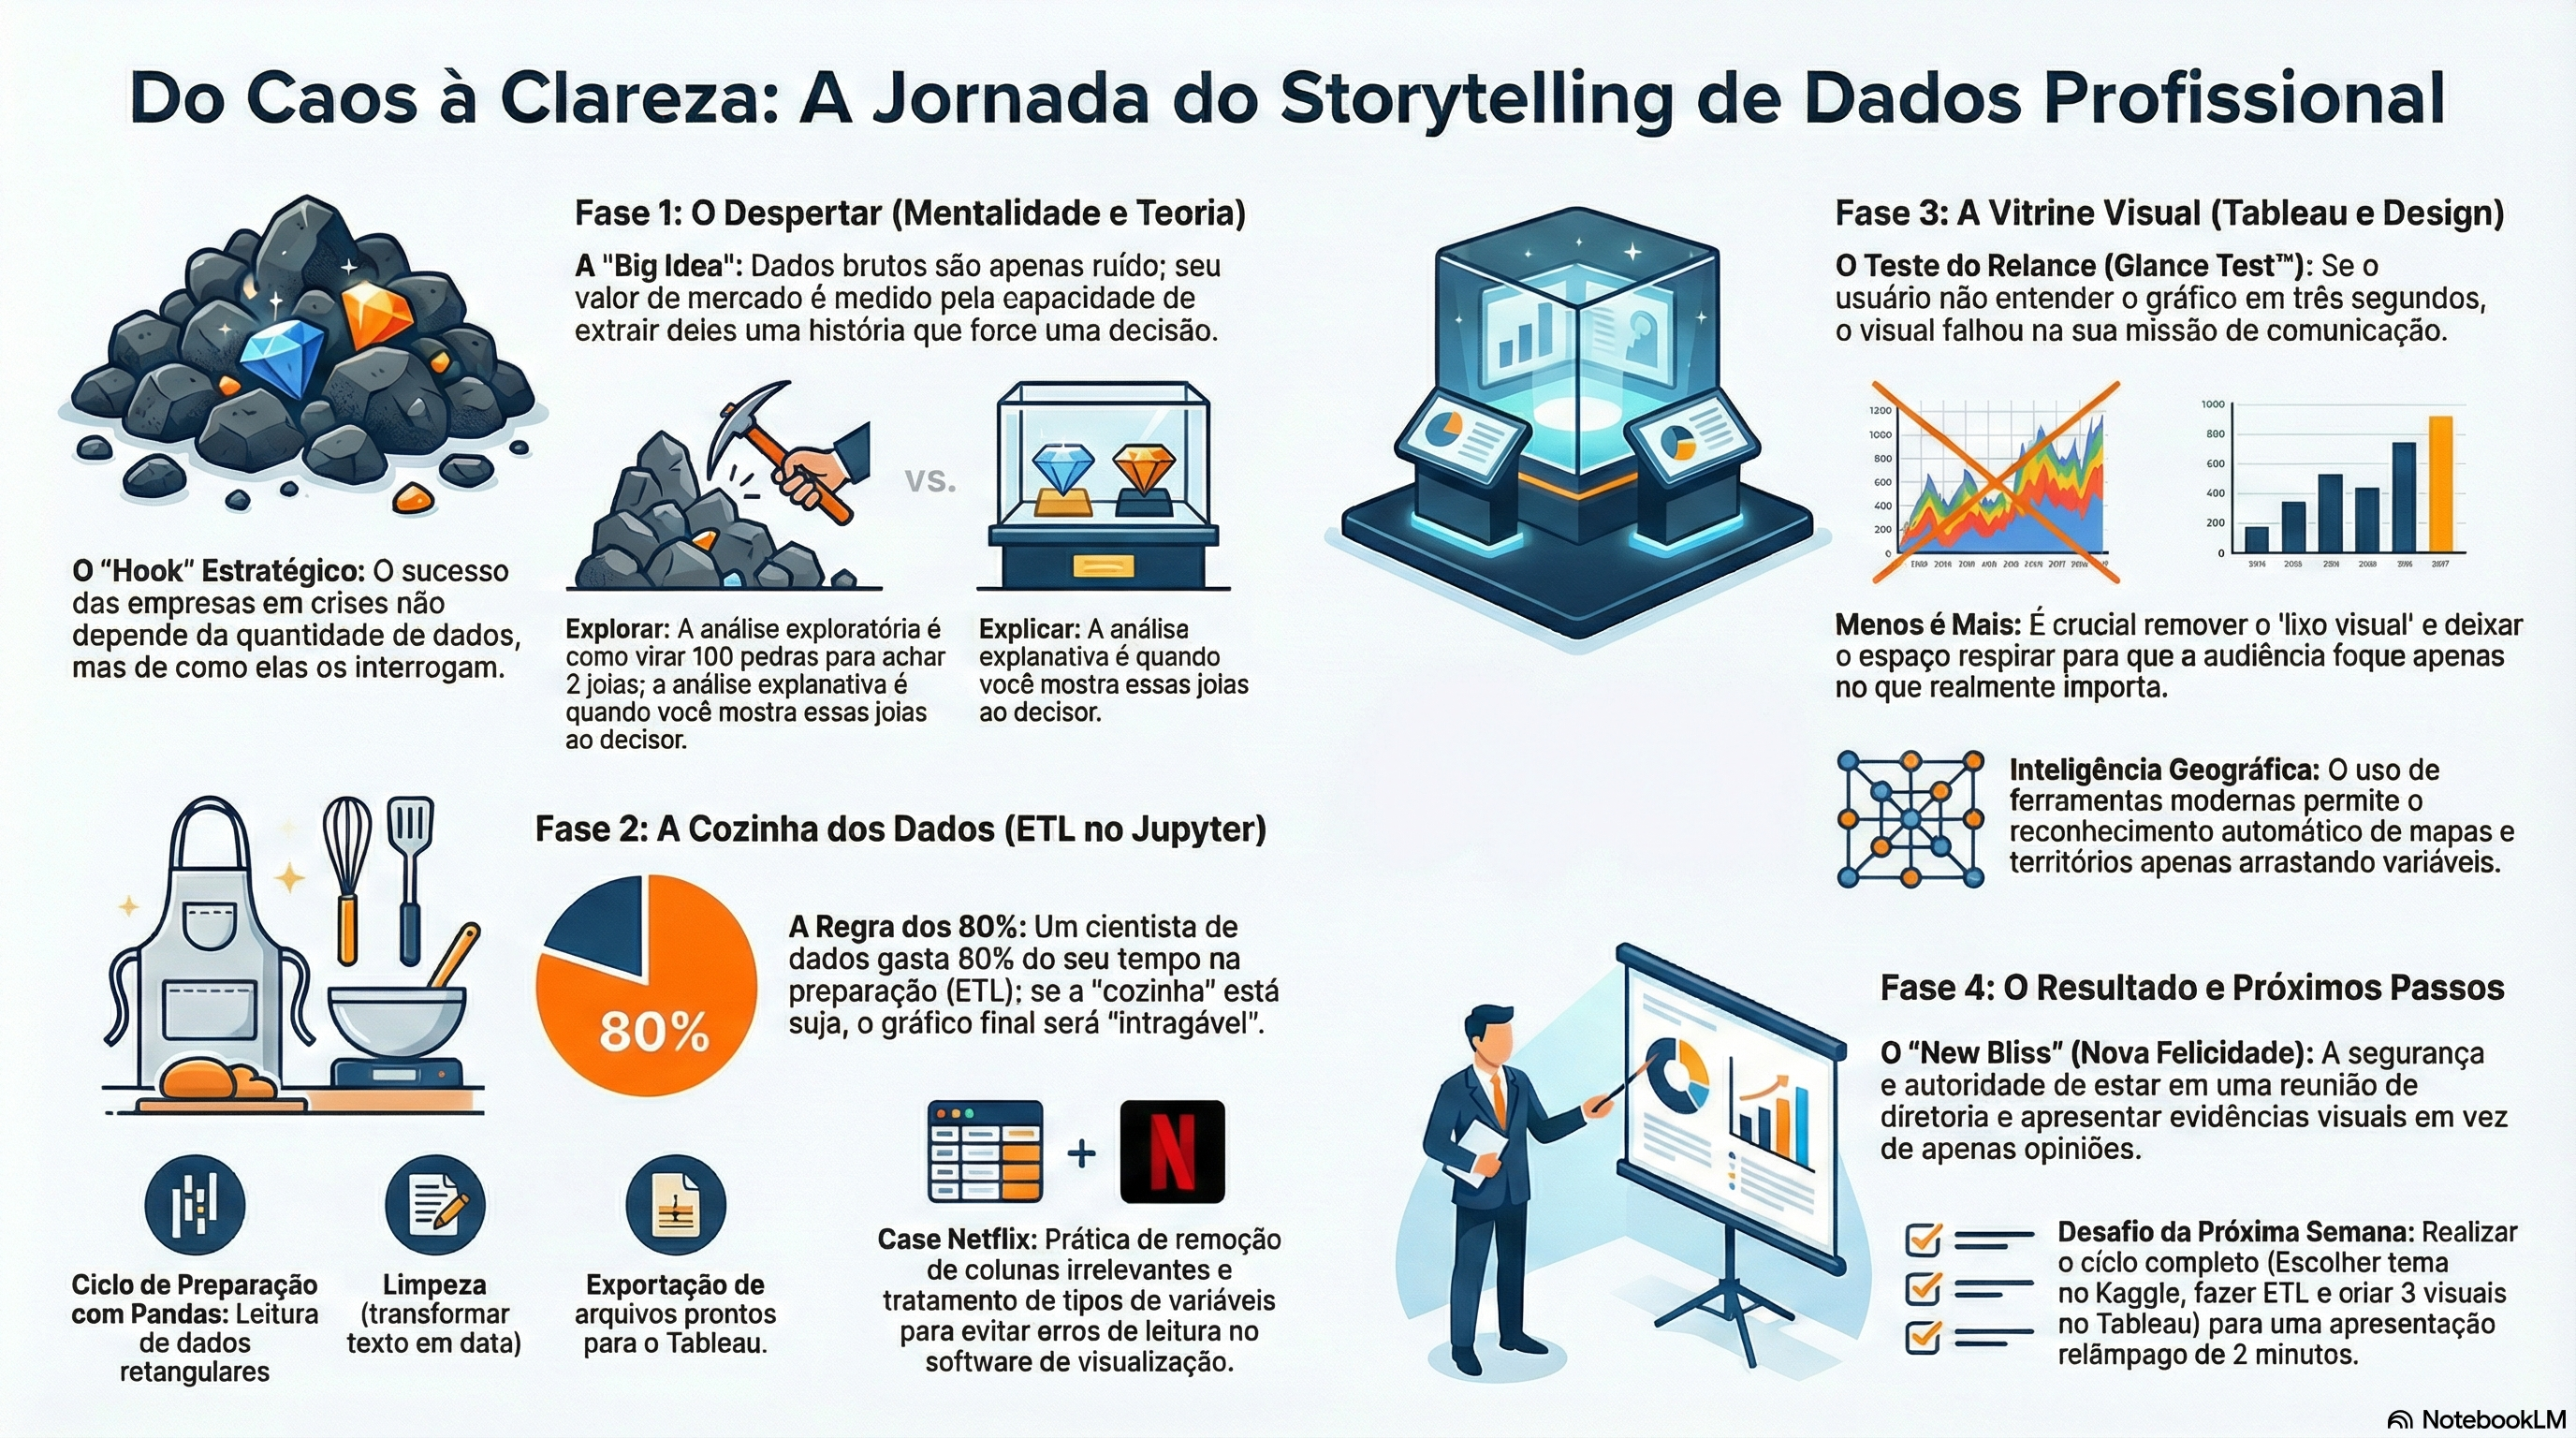
\includegraphics[width=0.92\textwidth]{semana01/info_semana1.png}
}{
  \fbox{\parbox{0.9\textwidth}{\centering \textit{(placeholder)}\quad Coloque aqui o arquivo \texttt{info\_semana1.png} em \texttt{aed/aula/semana01/}.}}
}
\end{center}

\section{Trabalho 1 (entrega na Semana 02) \textemdash{} 0,5 ponto na I unidade}
\subsection*{Objetivo pedagógico}
Cada aluno escolhe um tema e, além de \textbf{construir um infográfico}, ele precisa \textbf{estudar um pouco o assunto} (livro, PDF, artigos) e ensinar a turma em 10 minutos. 

\begin{SolvedBox}
\textbf{Formato (Semana 02):} cada aluno tem \textbf{10 minutos}.
\begin{itemize}[leftmargin=*]
  \item 7 min: construir/mostrar o infográfico (Tableau) e explicar a Big Idea.
  \item 3 min: explicar o que estudou (conceito) e responder 1 pergunta.
\end{itemize}

\textbf{Entregáveis:}
\begin{itemize}[leftmargin=*]
  \item 1 CSV (dataset escolhido) e 1 CSV limpo (separado);
  \item 1 notebook (ETL básico com evidência de limpeza real);
  \item 1 visual/infográfico no Tableau;
  \item 1 slide (ou texto curto) com \textbf{Big Idea} + 3 bullets de evidência.
\end{itemize}
\end{SolvedBox}

\subsection*{Os 20 temas (para eu mostrar no final da Semana 01)}
Eu apresento a lista e deixo claro: tema não é ``qualquer dataset''; tema é \textbf{uma pergunta + um recorte + um conceito para estudar}.

\begin{center}
\renewcommand{\arraystretch}{1.2}
\begin{tabular}{@{}c p{4.3cm} p{5.0cm} p{4.0cm}@{}}
\toprule
\textbf{\#} & \textbf{Tema (assunto)} & \textbf{Pergunta/recorte (para o infográfico)} & \textbf{Conceito para estudar} \\
\midrule
01 & Netflix: produções por ano & Houve crescimento? quais anos mudam o ritmo? & Eixo temporal e granularidade \\
02 & Netflix: filme vs série & Qual tipo domina? muda por ano? & Proporções e comparação \\
03 & Netflix: países mais presentes & Quais países lideram? e por quê? & Categóricas + limpeza de texto \\
04 & Netflix: classificação indicativa & Quais ratings mais comuns? & Distribuição categórica \\
05 & Netflix: gêneros (listed\_in) & Top gêneros e combinações & Categorias ``multivalor'' \\
06 & Vendas de videogames & Quais plataformas/regiões lideram? & Grupos e comparação \\
07 & Filmes (IMDb/TMDB) & Orçamento vs receita: existe relação? & Scatter e correlação (noção) \\
08 & Airbnb (NY) & Bairro vs preço: onde é mais caro? & Boxplot e dispersão \\
09 & Preços de abacate & Sazonalidade: meses mais caros? & Séries temporais \\
10 & Felicidade mundial & PIB vs felicidade: padrão global? & Correlação \neq causalidade \\
11 & Salários em Data Science & Senioridade vs salário: qual salto? & Segmentação por categoria \\
12 & Reviews e-commerce & Nota vs recomendação: o que pesa? & Viés de seleção \\
13 & Starbucks nutrição & Calorias vs tamanho: onde está o pico? & Outliers e interpretação \\
14 & Qualidade do vinho & \% álcool vs qualidade: há tendência? & Relação bivariada \\
15 & Diabetes (Pima) & Glicose vs diagnóstico: separa grupos? & Comparar distribuições \\
16 & Crimes (cidade) & Horário/dia: onde estão os picos? & Heatmap simples \\
17 & Apps (Google Play) & Avaliação vs installs: existe padrão? & Escalas e log (noção) \\
18 & Temperatura global & Tendência: aquecimento aparece? & Linha do tempo e smoothing \\
19 & Spotify top hits & BPM vs popularidade: existe relação? & Dispersão e clusters \\
20 & Titanic & Sobrevivência por classe/sexo: qual diferença? & Proporções e narrativa \\
\bottomrule
\end{tabular}
\end{center}

\begin{NoteBox}
Eu deixo o aluno escolher um tema, mas eu cobro que ele traga \textbf{uma Big Idea} e \textbf{uma evidência} (não apenas um gráfico bonito). Eu reforço que o objetivo é ensinar a turma.
\end{NoteBox}

\section{Referências (para eu citar e orientar leitura)}
Eu menciono explicitamente os materiais e deixo a turma saber que eles vão reaparecer na unidade:
\begin{itemize}[leftmargin=*]
  \item Estatística prática e AED (base): \cite{bruce_estatistica_pratica}.
  \item Storytelling (clareza, Big Idea, persuasão): \cite{duarte_datastory}.
  \item Apostila/guia LaTeX (conteúdos e exercícios): \cite{unifacol_apostila_aed}.
\end{itemize}

\chapter{Semana 02 (09/02--11/02) --- Trabalho 1 + Dados retangulares}

\section{Objetivo da semana}
Nesta semana eu executo duas coisas em paralelo: (1) \textbf{avaliar} a entrega curta do Trabalho 1 (vale 0,5 ponto na I unidade); (2) consolidar a base de \textbf{dados retangulares} e qualidade de dados.

\section{Roteiro (19h--22h)}
\begin{itemize}[leftmargin=*]
  \item \textbf{19:00--20:00} --- Apresentações do Trabalho 1 (no máximo 1h).
  \item \textbf{20:00--21:20} --- Teoria + prática: dados retangulares, dicionário de dados, tipos, ausências, duplicadas.
  \item \textbf{21:20--22:00} --- Mini-lab: refazer o ETL com checklist e exportar CSV limpo.
\end{itemize}

\section{Entrega (Trabalho 1 --- 0,5 ponto na I unidade)}
\begin{SolvedBox}
\textbf{Formato:} cada aluno tem \textbf{10 minutos} para construir um infográfico/visual (com base no tema escolhido na Semana 01) e explicar para a turma.

\textbf{Artefatos:}
\begin{itemize}[leftmargin=*]
  \item 1 dataset (CSV) escolhido dentre os 20 temas;
  \item 1 ETL básico em Python (notebook) com pelo menos 1 limpeza real;
  \item 1 infográfico no Tableau (ou 1 dashboard simples);
  \item 1 slide/texto com \textbf{Big Idea} + 3 bullets de evidência.
\end{itemize}

\textbf{Critério:} clareza (Teste do Relance), coerência do recorte e conclusão ligada a decisão.
\end{SolvedBox}

\section{Próximo passo}
Depois que os alunos apresentarem, eu conecto o que eles trouxeram com o conceito de \textbf{tabela retangular} e com o que vai cair na Prova I Unidade.

\chapter{Semana 03 (23/02--25/02) --- Estatística descritiva I (posição)}

\section{Objetivo da semana}
Eu ensino medidas de posição (média, mediana, moda) com foco na intuição e em como isso vira insight na AED.

\section{Conteúdo}
\begin{itemize}[leftmargin=*]
  \item Média, mediana e moda: quando usar.
  \item Resumos com Pandas (\texttt{describe}, \texttt{value\_counts}, \texttt{groupby}).
  \item Leitura crítica: assimetria e outliers.
\end{itemize}

\section{No quadro (exemplo)}
\begin{BoardBox}
\textbf{Eu escrevo:}
\[\bar{x}=\frac{1}{n}\sum_{i=1}^{n}x_i\qquad\tilde{x}=\text{valor central (dados ordenados)}\]
\end{BoardBox}

\chapter{Semana 04 (02/03--04/03) --- Trabalho 2 + Variabilidade}

\section{Ritmo da aula}
\begin{itemize}[leftmargin=*]
  \item \textbf{Até 1h}: apresentações do Trabalho 2.
  \item \textbf{Restante}: variância, desvio-padrão, IQR, boxplot.
\end{itemize}

\section{Entrega (Trabalho 2)}
\begin{SolvedBox}
Mini-relatório AED (posição + dispersão) + 2 visuais (boxplot + histograma) + Big Idea.
\end{SolvedBox}

\chapter{Semana 05 (09/03--11/03) --- Distribuições e dados ausentes}

\section{Objetivo da semana}
Eu ensino o aluno a ler o ``formato'' dos dados (histograma, caudas, assimetria) e a tomar decisões sobre missing.

\section{Conteúdo}
\begin{itemize}[leftmargin=*]
  \item Histogramas e leitura de distribuição.
  \item Missing: remover, imputar, sinalizar.
  \item Preparar dados para viz (tipos, categorias, datas).
\end{itemize}

\chapter{Semana 06 (16/03--18/03) --- Trabalho 3 + Correlação}

\section{Ritmo da aula}
\begin{itemize}[leftmargin=*]
  \item \textbf{Até 1h}: apresentações do Trabalho 3.
  \item \textbf{Restante}: correlação, scatter, leitura sem causalidade.
\end{itemize}

\section{Entrega (Trabalho 3)}
\begin{SolvedBox}
Diagnóstico (missing + outliers + distribuição) + 1 relação bivariada (scatter) + Big Idea.
\end{SolvedBox}

\chapter{Semana 07 (23/03--25/03) --- Categóricas e revisão para Prova I}

\section{Objetivo da semana}
Eu fecho a Unidade I, consolidando leitura de variáveis categóricas e revisão guiada.

\section{Conteúdo}
\begin{itemize}[leftmargin=*]
  \item Tabelas de frequência e proporções.
  \item Gráficos de barras e escolhas de visual.
  \item Revisão para Prova I Unidade.
\end{itemize}

\chapter{Semana 08 (20/04) --- Trabalho 4 + Storytelling}

\section{Observação do calendário}
Aula concentrada (apenas segunda-feira).

\section{Ritmo da aula}
\begin{itemize}[leftmargin=*]
  \item \textbf{Até 1h}: apresentações do Trabalho 4.
  \item \textbf{Restante}: Big Idea, storyboard e narrativa.
\end{itemize}

\section{Entrega (Trabalho 4)}
\begin{SolvedBox}
Roteiro curto (Big Idea + 3 evidências) + wireframe de dashboard + 1 visual no Tableau.
\end{SolvedBox}

\chapter{Semana 09 (27/04--29/04) --- Design de informação}

\section{Objetivo da semana}
Eu ensino como transformar um visual correto em um visual \textbf{claro}, com hierarquia e consistência.

\section{Conteúdo}
\begin{itemize}[leftmargin=*]
  \item Teste do Relance (título-mensagem).
  \item Hierarquia visual: cor, espaço em branco, alinhamento.
  \item Padrões para dashboards.
\end{itemize}

\chapter{Semana 10 (04/05--06/05) --- Trabalho 5 + Tableau interativo}

\section{Observação do calendário}
06/05 é feriado (Vitória de Santo Antão): ajustar dinâmica para caber no tempo.

\section{Ritmo da aula}
\begin{itemize}[leftmargin=*]
  \item \textbf{Até 1h}: apresentações do Trabalho 5.
  \item \textbf{Restante}: filtros, parâmetros, ações e interatividade.
\end{itemize}

\section{Entrega (Trabalho 5)}
\begin{SolvedBox}
Dashboard com 1 a 2 mecanismos de interatividade + título-mensagem + checklist do Teste do Relance.
\end{SolvedBox}

\chapter{Semana 11 (11/05--13/05) --- Dashboards que forçam decisão}

\section{Objetivo da semana}
Eu ajudo o aluno a organizar narrativa + layout + consistência de métricas, pensando em decisão e próximo passo.

\section{Conteúdo}
\begin{itemize}[leftmargin=*]
  \item Estrutura: contexto, diagnóstico e recomendação.
  \item Consistência de definições.
  \item Pitch de 3 minutos.
\end{itemize}

\chapter{Semana 12 (18/05--20/05) --- Trabalho 6 + Fechamento}

\section{Ritmo da aula}
\begin{itemize}[leftmargin=*]
  \item \textbf{Até 1h}: apresentações do Trabalho 6.
  \item \textbf{Restante}: refinamento, revisão e checklist para Prova II.
\end{itemize}

\section{Entrega (Trabalho 6)}
\begin{SolvedBox}
Dashboard final + pitch (3 min) + checklist completo (dados limpos + Big Idea + interatividade).
\end{SolvedBox}


\printbibliography
\end{document}
